%\documentclass[aspectratio=169]{beamer}
\documentclass{beamer}
\usetheme{PaloAlto}
%\usetheme{AnnArbor}
\setbeamercovered{transparent}

\usepackage[utf8]{inputenc}

\title{Curso de BEAMER.}
\author[Felipe]{Felipe F. Soares.}
\institute[UFC]{Universidade Federal do Ceará \\ ufc.br}
\date{2016}
%\date{}
%\date{Nome do evento, 2016}
\logo{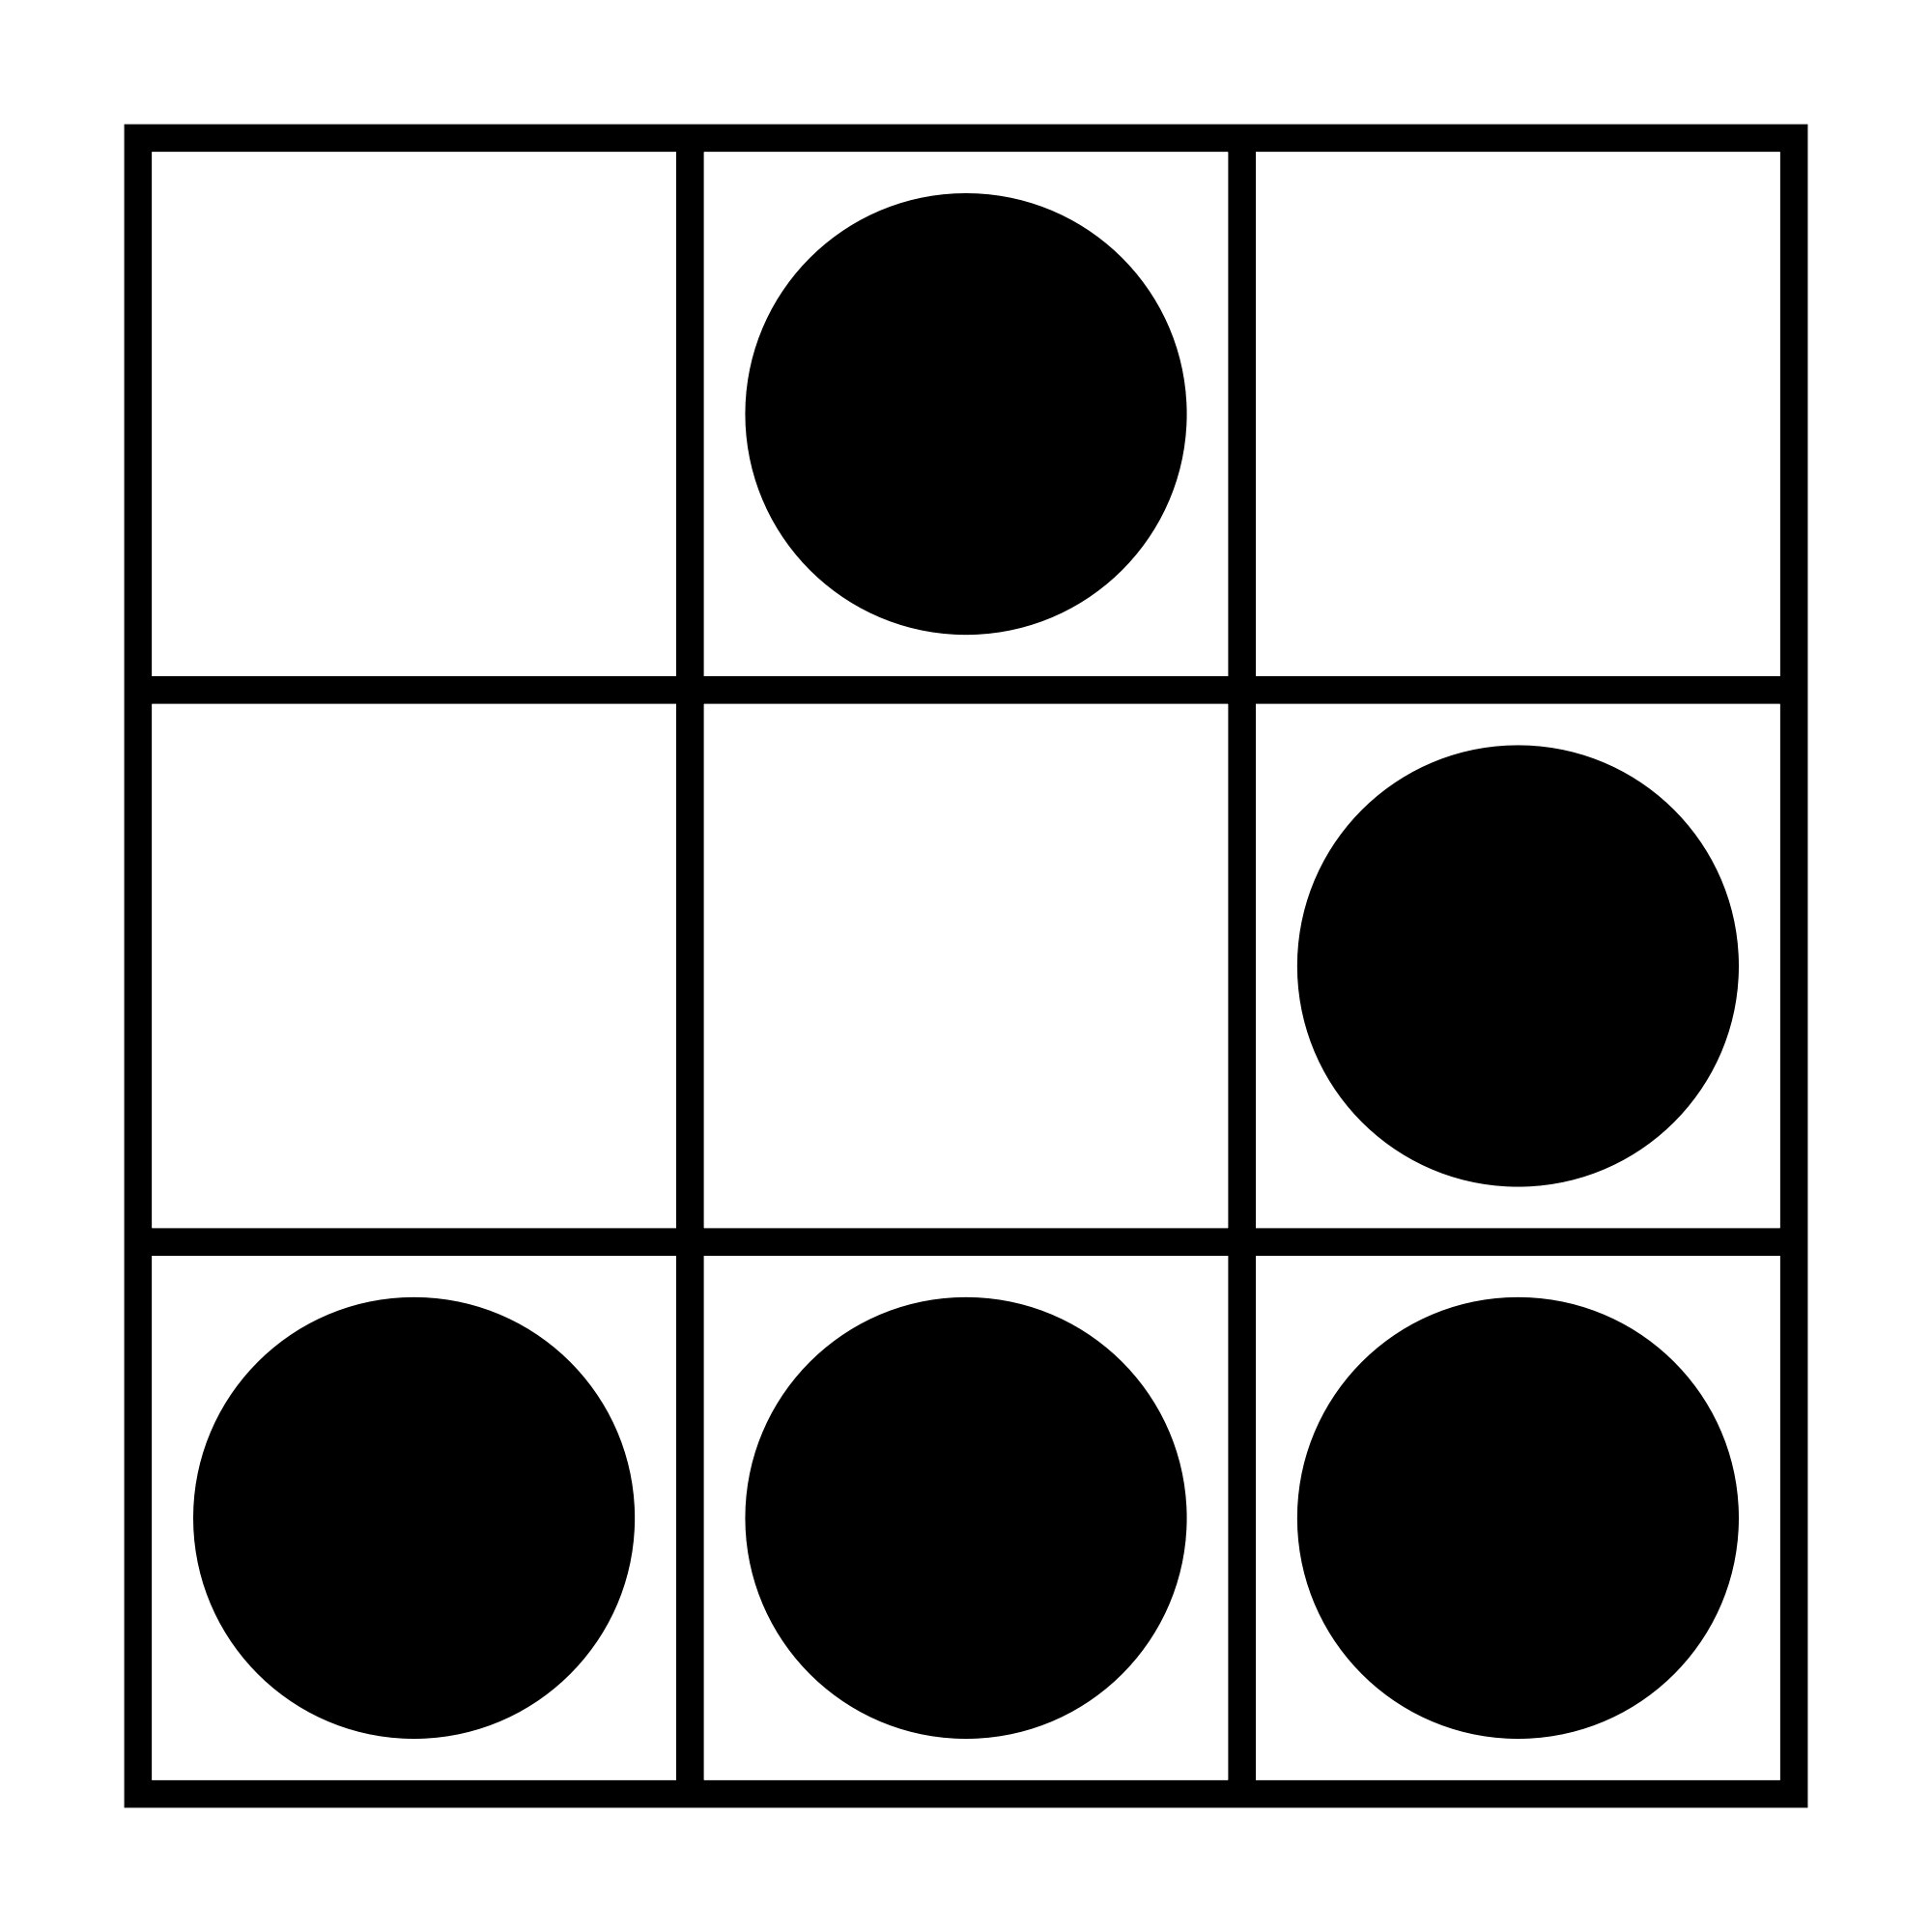
\includegraphics[scale=0.01]{images/glider.png}}

\begin{document}
	\begin{frame}{Esse é o título do quadro}
		\titlepage
	\end{frame}
	
	\begin{frame}
		\frametitle{Esse é o título do quadro uncover}
		\framesubtitle{Esse é o subtítulo}
		
		\uncover<1->{Vamos resolver uma equação do segundo grau:
		$$ax^2 + bx + c = 0$$ }
		
		\uncover<2->{Primeiro identifique os coeficientes $a$, $b$ e $c$.}
		
		\uncover<3>{Em seguida, calcule o valor de :
		$$\Delta = b^2 - 4ac$$}
		
		\uncover<4>{Calcule a primeira raiz:
		$$x_1 = \frac{-b + \sqrt{\Delta}}{2a}$$}
		
		\uncover<5>{Calcule a segunda raiz:
		$$x_2 = \frac{-b - \sqrt{\Delta}}{2a}$$}
		
	\end{frame}
	
	\begin{frame}
		\frametitle{Esse é o título do quadro visible}
		\framesubtitle{Esse é o subtítulo}
		
		\visible<1>{Vamos resolver uma equação do segundo grau:
		$$ax^2 + bx + c = 0$$ }
		
		\visible<2>{Primeiro identifique os coeficientes $a$, $b$ e $c$.}
		
		\visible<3>{Em seguida, calcule o valor de :
		$$\Delta = b^2 - 4ac$$}
		
		\visible<4>{Calcule a primeira raiz:
		$$x_1 = \frac{-b + \sqrt{\Delta}}{2a}$$}
		
		\visible<5>{Calcule a segunda raiz:
		$$x_2 = \frac{-b - \sqrt{\Delta}}{2a}$$}
		
	\end{frame}
	
	\begin{frame}
		\frametitle{Esse é o título do quadro only}
		\framesubtitle{Esse é o subtítulo}
		
		\only<1>{Vamos resolver uma equação do segundo grau:
		$$ax^2 + bx + c = 0$$ }
		
		\only<2>{Primeiro identifique os coeficientes $a$, $b$ e $c$.}
		
		\only<3>{Em seguida, calcule o valor de :
		$$\Delta = b^2 - 4ac$$}
		
		\only<4>{Calcule a primeira raiz:
		$$x_1 = \frac{-b + \sqrt{\Delta}}{2a}$$}
		
		\only<5>{Calcule a segunda raiz:
		$$x_2 = \frac{-b - \sqrt{\Delta}}{2a}$$}
		
	\end{frame}
\end{document}